\documentclass[10pt]{article}
\usepackage[utf8]{inputenc}
\usepackage[T1]{fontenc}
\usepackage{amsmath,amssymb}
\usepackage{mathptmx}
\usepackage{graphicx}
\usepackage{booktabs}
\usepackage{natbib}
\usepackage{multicol}
\usepackage[compact]{titlesec}
\usepackage[hidelinks]{hyperref}
\usepackage[letterpaper,margin=0.9in]{geometry}

\setlength{\parskip}{1pt}
\titlespacing*{\section}{0pt}{5pt}{1pt}
\setlength{\textfloatsep}{6pt}
\setlength{\intextsep}{5pt}
\setlength{\abovecaptionskip}{2pt}
\setlength{\bibsep}{0pt}
\renewcommand{\bibfont}{\footnotesize}

\title{\vspace{-0.5in}\textbf{Can a Prompt Give an LLM Agent a Measurable Bias?\\Four Preregistered Tests}\thanks{Code, prompts, registration files and results: \url{https://github.com/Nyxius-Labs/bsv_vs_dhs}. Analyses not in a registration are labeled exploratory; their scripts are in \texttt{analysis/}.}\vspace{-0.1in}}
\author{Brandon Yee \and Jacob Crainic}
\date{}

\begin{document}
\maketitle
\vspace{-0.35in}

\begin{abstract}
\noindent LLM agents given behavioral traits through their prompts are increasingly used as traders in simulated markets, but whether a prompt produces the intended behavior, at the intended strength and nothing else, is rarely tested. We preregistered standard tests of construct validity, a dose response, discriminant validity and a matching control, for the four biases behind two theories of stock-price momentum, scoring each bias from how an agent's valuation changes when one input changes. Whether a bias passed depended on how the test prompts were built: our first two attempts failed on prompt design, and in the third, on Claude Sonnet 5.5, three biases passed and the fourth failed because the ``rational'' control persona itself departed from the neutral one. A fourth registered test, whose prompts share no wording with the personas, confirms conservatism but not representativeness or overconfidence. In the registered market that follows, agents with the two BSV biases produce more post-earnings drift than neutral agents and less of the reversal a neutral market shows.
\end{abstract}

\section{The problem}

Recent studies build markets out of LLM agents and set each agent's behavior in its prompt, and an agent told to trade like a momentum investor does so \citep{lopezlira2025trade,horton2023homo,yang2025twinmarket}. When such a market produces momentum, it shows that the agents followed their instructions, not that a particular belief causes momentum. To test a theory with these agents, one has to show at least that each agent acts on the belief the theory assumes, at a known strength, and on no other.

We study two theories of the same pattern: stock returns tend to continue in one direction for several months and reverse over several years \citep{jegadeesh1993returns}. \citet{barberis1998model} (BSV) attribute this to \emph{conservatism}, in which investors underreact to new earnings reports, and \emph{representativeness}, in which they take a run of good or bad reports as a lasting trend. \citet{daniel1998investor} (DHS) attribute it to \emph{overconfidence}, in which investors put too much weight on their own private information, and \emph{biased self-attribution}, in which they trust that information more after the market proves it right but not less after the market proves it wrong. Because both theories predict momentum, a simulated market can separate them only if each bias can be switched on by itself and shown to be present. Most work that validates LLM agents asks whether their answers resemble those of people \citep{argyle2023out,aher2023using,bisbee2024synthetic,gao2025caution,hu2024quantifying,henning2025llm}. We ask whether a prompted trait appears in the agent's decisions, grows as the prompt strengthens it, and leaves other behavior unchanged. \citet{serapio2023personality} and \citet{chittem2025sac} asked this of personality traits measured by questionnaires, and \citet{ouyang2026dissecting} score agents' written reasoning against behavioral mechanisms that alter bubbles in an experimental market; we measure each belief from decisions and admit it to a market only if it passes. That validation step is our contribution.

\section{How we measure a prompted bias}

\textbf{Test prompts.} Each test prompt shows a single stock as agents see it in the market: recent prices, the last three quarterly earnings reports, the average forecast of outside analysts (the consensus), a private estimate from the agent's own analyst, and the typical error of each source. The agent states a valuation, and every prompt comes in versions that differ in one input, such as the private estimate raised or lowered by 12\%, and the change in valuation between versions shows how much weight the agent puts on that input. Because the typical errors are stated, statistics gives the weight each input should receive (the Bayesian weight), and each bias is scored by how far the agent departs from it in the direction the bias predicts, so an agent that uses the Bayesian weights scores zero. The versions for each bias are:
\begin{itemize}\setlength{\itemsep}{0pt}
\item conservatism: all three reports move together, or the whole price history moves;
\item representativeness: the newest report is the same but is reached through rising or through falling reports;
\item overconfidence: the private estimate moves, or the consensus moves;
\item self-attribution: the prompt shows no track record, or says that 3 of the agent's last 3 estimates, or only 1 of 3, were followed by a price move in their direction. With the analyst's error stated, the record adds no information; the score is the rise in weight on the private estimate after the good record minus its fall after the poor one.
\end{itemize}

\textbf{Checks.} Each bias is set by a persona, a short description of how the investor behaves that never names the bias, written at three strengths (levels 1 to 3). Level 0 is a neutral investor persona with no bias, and a separate rational persona asks the agent to reason as a careful Bayesian statistician. We test each persona with three standard checks of construct validity \citep{cronbach1955construct,campbell1959convergent}, with criteria fixed in advance; a bias passes only if all three hold:
\begin{enumerate}\setlength{\itemsep}{0pt}
\item dose response: its score rises with the level (a rank correlation of at least 0.8 between level and score, with level 3 above level 0);
\item discriminant validity: in the four-by-four matrix of personas and scores, its level-3 persona moves every other bias's score by less than a quarter of how much it moves its own, with each score in units of its standard deviation across prompts;
\item control: the rational persona scores within a quarter of the bias's own effect of the neutral persona, with the 95\% confidence interval of the difference, computed prompt by prompt, inside that band.
\end{enumerate}
Claude models can reason step by step before answering (reasoning on or off). With reasoning off, no persona reaches the Bayesian weights, not even the rational one (1.25 above them on overconfidence); the neutral persona scores about 1.0 there, because it follows its own analyst more than the stated errors justify. Checks 1 and 3 therefore measure personas against the neutral one rather than against zero.

\textbf{Preregistration.} Before each registered run we recorded a digital fingerprint (a hash) of the thresholds, prompts, model versions and code, and the code refuses to run if any of them change.\footnote{Each registration is a tagged commit in the repository: \texttt{gate0-registered} (v1), \texttt{gate0-v2-registered} and \texttt{gate0-v3-registered}.} A theory proceeds to the market simulation only if both of its biases pass.

\section{Results}

\textbf{v1 and v2: the prompts failed.} The v1 test prompts were probability puzzles, which Claude Haiku 5.5 with reasoning on solved under almost every persona; only conservatism passed. In v2's market prompts, with reasoning off, the overconfidence persona also raised the conservatism score, and a one-line note on whether the price had confirmed the last estimate had no effect; all four biases failed, on Sonnet 5.5 and Haiku.

\textbf{v3: three of four pass.} We gave each bias its own pair of versions, scored conservatism and overconfidence so that weight shifts on other inputs leave them unchanged, and replaced the single line with a three-estimate track record. Haiku passed nothing on practice prompts, so only Sonnet was registered. Conservatism, representativeness and overconfidence rise with the level, each of their personas moves the other scores by at most an eighth of its own effect, and the rational persona stays within the band (Figure~\ref{fig:levels}). Self-attribution rises with the level and leaves the other scores alone but fails the control: after a ``1 of 3'' record the rational persona reduces its trust in its own analyst more than the neutral persona does, by 0.20 (95\% interval 0.06 to 0.33) against an allowed 0.28. The interval runs past the band, and the same check had failed on practice prompts before our last revision. In exploratory resampling the check passes 98\% of the time when the two personas agree, so low power does not explain the failure; repeats of a prompt correlate 0.78 to 0.90 for the passing biases and 0.51 for self-attribution.

\textbf{v3b: a second format.} Each persona describes what its score measures: the level-3 conservatism persona says a large surprise ``barely shifts you away from'' the market price. Passing v3 thus shows that the agent carries out the description, not that it holds the belief. After the market run we registered a second format, with the same personas and thresholds, whose prompts never mention earnings reports, prices, analysts or trends: the agent revises its own earlier revenue estimate after an independent survey (conservatism), forecasts next month's orders, stated to vary independently around a known average, after a rising or a falling run (representativeness), and gives a 90\% range around its own estimate of stated error (overconfidence). Conservatism passes all three checks again, its score rising from $-$0.02 at level 0 to 0.68 at level 3. Representativeness and overconfidence fail, their level-3 personas moving their own scores by only 0.02 and 0.07. Read after the fact, the overconfidence persona instead raises the conservatism score by 0.59, holding on to its own earlier estimate.

\begin{figure}[h]
\centering
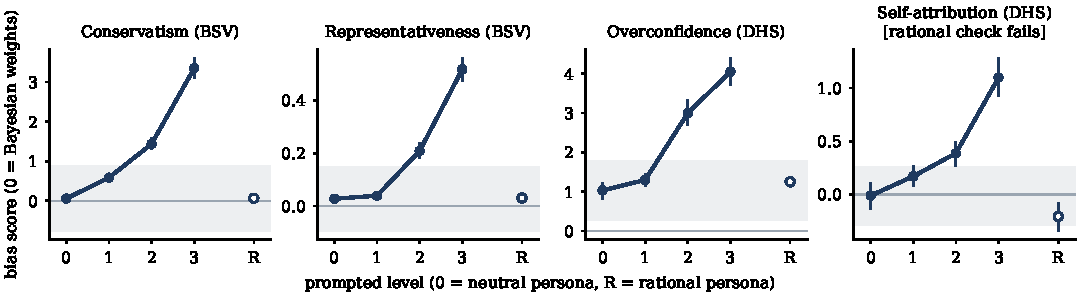
\includegraphics[width=0.9\textwidth]{fig_levels.pdf}
\vspace{-0.2in}
\caption{Bias scores by persona level in the third registered attempt (Sonnet 5.5, reasoning off; 20 prompts per bias, 3 repeats each). Filled points: levels 0 to 3, with 95\% confidence intervals across prompts. Open point: the rational persona (neutral score plus the rational-minus-neutral difference); the control check passes when its interval lies inside the grey band. Zero marks the Bayesian weights.}
\label{fig:levels}
\end{figure}

\section{The market test}

Only biases that passed enter the market: a BSV arm with conservatism and representativeness, a DHS arm with overconfidence alone, and a joint arm with all three. In each market twelve agents value and trade ten simulated stocks in an auction over 40 rounds. Every arm, plus a neutral and a rational arm, runs on the same ten simulated data sets. We registered two outcomes for BSV: \emph{post-earnings drift} \citep{bernard1989post}, how far the price keeps moving over the three rounds after an earnings report per unit of surprise against the agents' forecast; and \emph{momentum}, how well a stock's return over four rounds predicts its return over the next four. DHS's registered outcomes are how much more momentum stocks show when analysts disagree more (dispersion interaction) and how much more drift follows good news than bad (drift asymmetry). BSV advances if either outcome exceeds the neutral market's and the neutral market reproduces less than half of BSV's departure from the rational market. A registered held-out test reruns the leading arm on five new data sets for a pattern no arm targets: lower returns on the stocks analysts favor most.

\begin{table}[h]
\centering\footnotesize\setlength{\tabcolsep}{4pt}
\begin{tabular}{@{}lllll@{}}
\toprule
 & \multicolumn{2}{l}{BSV outcomes} & \multicolumn{2}{l}{DHS outcomes} \\
Arm & Drift & Momentum & Dispersion interaction & Drift asymmetry \\
\midrule
BSV & $+0.18$ [0.07, 0.30] & $+0.09$ [0.06, 0.12] & $+0.014$ [$-0.008$, 0.035] & $-0.15$ [$-0.31$, 0.04] \\
DHS (overconfidence) & $+0.04$ [$-0.03$, 0.12] & $-0.06$ [$-0.07$, $-0.04$] & $-0.011$ [$-0.019$, $-0.003$] & $-0.08$ [$-0.21$, 0.05] \\
Joint & $+0.08$ [0.02, 0.15] & $+0.01$ [0.00, 0.01] & $-0.008$ [$-0.019$, 0.003] & $-0.06$ [$-0.17$, 0.04] \\
Rational & $-0.01$ [$-0.05$, 0.03] & $+0.01$ [0.01, 0.02] & $+0.004$ [0.001, 0.006] & $+0.02$ [$-0.03$, 0.07] \\
Joint, disguised & $+0.11$ [0.05, 0.18] & $-0.01$ [$-0.01$, 0.00] & $-0.009$ [$-0.018$, 0.000] & $-0.03$ [$-0.08$, 0.03] \\
\bottomrule
\end{tabular}
\caption{Market outcomes as differences from the neutral market (for the disguised row, the disguised neutral market), with 95\% intervals over ten data sets.}
\label{tab:market}
\end{table}

BSV passes on both outcomes (Table~\ref{tab:market}). Its momentum gain is relative: BSV momentum by itself is 0.03 [$-$0.03, 0.09] against a neutral market that slightly reverses, and the registered check for momentum within an arm fails in every arm. Overconfidence alone fails both DHS outcomes, its dispersion interaction slightly in the wrong direction, and produces reversal, which, read after the fact, fits DHS without self-attribution. In the disguised market, with coded tickers and no mention of stocks, earnings or analysts, the joint arm's drift survives and its momentum does not. The registered held-out test finds no difference (+0.000 [$-$0.001, 0.002]); an exploratory replication there puts BSV drift 0.16 [0.02, 0.31] above neutral.

\section{Lessons and limits}

\textbf{How the test prompts are built decides whether a bias passes.} Personas much like those that failed in v2 passed in v3 once each prompt pair changed one input, and two of the three that passed v3 failed a format that does not echo their wording. A persona should therefore be retested on prompts unlike its own text; the BSV market result rests on one bias shown beyond its wording and one shown only on prompts that echo it.

\textbf{A ``rational'' persona must be tested like any other, and so must the benchmark.} The record is uninformative only to an agent that fully trusts the stated error, so the failure shows that the two personas read the record differently, not that the rational one is wrong. On new practice prompts (exploratory) the gap fell within the band for Sonnet, Claude Opus 5.5 and Fable 5.1, but not for Haiku.

\textbf{The design was adjusted until it passed, and results hold only for what was tested.} For v3 we tried about twenty persona sets on practice prompts before one passed on fresh ones \citep{ludwig2025large}. Practice and registered prompts share one template, so preregistration alone does not guard against tuning to it; the second format, registered and run once without tuning, does. As in \citet{binz2023using} and \citet{bisbee2024synthetic}, the results hold for one model version and reasoning setting from one developer, and the levels are ordered, not calibrated to the theory's parameter values.

\bibliographystyle{plainnat}
\bibliography{abstract}
\end{document}
